\section{Causal-Order Broadcast}
Uniform reliable broadcast doesn't deal with the order in which the
message are deliver. The causal-order broadcast remedy to this
problem.

\paragraph{}
We have the relation $m_1 \to m_2$ ($m_1$ causally precedes $m_2$) if
\begin{itemize}
    \item FIFO order: Some process $p_i$ broadcasts $m_1$ before
        broadcasting $m_2$
    \item Network order: Some process $p_i$ delivers $m_1$ and
        later broadcasts $m_2$
    \item Transitivity: There is a message $m'$ s.t $m_1 \to m' \ and \ m'\to m_2$
\end{itemize}
\paragraph{Property}
\begin{itemize}
    \item \textbf{CB:} If node $p_i$ delivers $m_1$, then $p_i$ must have
        delivered every message causally preceding ($\to$) $m_1$ before $m_1$.
    \item \textbf{CB':} If $p_j$ delivers $m_1$ and $m_2$, and $m_1\to m_2$
        then $p_j$ must deliver $m_1$ berfore $m_2$.
\end{itemize}

\begin{figure}[!ht]
    \centering
    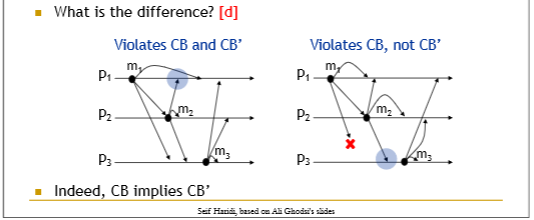
\includegraphics[scale=0.8]{img/cbs_properties.png}
\end{figure}
\FloatBarrier{}

\subsection{Implementation}
The idea is to broadcast the message along with its history (message
that were sent before it). This history is an ordered list of
causally preceding messages called $past_m$

\begin{lstlisting}[caption={Fail-Silent Reliable Causal Order broadcast}, mathescape, captionpos=b]
upon event <Init> do
    delivered := $\emptyset$
    past := nil

upon event <rcoBroadcast | m> do
    trigger <rbBroadcast | (DATA, past, m)>
    past := append(past, <$p_i$, m>)

upon event <rbDeliver | $p_i$, (DATA, past$_m$, m)> do
    if m $\notin$ delivered then
        forall ($s_n$, n) $\in$ $past_m$ do                         // in ascending order
            if n $\notin$ delivered then
                trigger <rcoDeliver | $s_n$, n>        // deliver preceding messages
                delivered := devilered $\cup$ {n}
                past := append(past, <$s_n$, n>) // append to history
        trigger <rcoDeliver | $p_i$, m>               // deliver current message
        delivered := delivered $\cup$ {m}
        past := append(past, <$p_i$, m>)              // append to history
\end{lstlisting}


\subsubsection{First algorithm}
The problem with this algorithm is that the size of the message
grows. The idea to improve the algorithm is to detect with
ack when all correct nodes got the message and delete from
past if it's the case (Garbage Collector). \newline

This algorithm is bad because the $ack[m]$ array also grows with time and the
garbage collector can't work with a $\Diamond P$.

\begin{lstlisting}[caption={Garbage Collected Causal Order Broadcast}, mathescape]
upon event <Init> do
    delivered := $\emptyset$
    past := nil
    correct := $\Pi$
    forall m:
        ack[m] := $\emptyset$  // bookkeeping of acks

upon event <crash | $p_i$> do
    correct := correct \ {$p_i$}

upon event m $\in$ delivered AND seld $\notin$ ack[m] do // called upon coDeliver
    ack := ack[m] $\cup$ {self}
    trigger <rbBroadcast | (ACK, m)>  // ack to all

upon event <rbDeliver | $p_i$, [ACK, m]> do
    ack := ack[m] $\cup$ {$p_i$}
    if correct $\subseteq$ ack[m] do
        past := remove(past, <x, m>)  // When received ack from all, GC m from any x
\end{lstlisting}


%TODO Question on GC

\subsubsection{Second algorithm}
In the first algorithm, the history was a list, in this one it's a
\textbf{vector timestamp} (vector clock). \newline
Each node has a vector clock s.t a node $p_i$:
\begin{itemize}
    \item VC[i]: number of messages $p_i$ coBroadcasted
    \item VC[j], $j \neq i$: number of messages $p_i$ coDelivered from $p_j$
\end{itemize}
The delivery of $m$ is only done if $VC_m$ (attached VC) precedes $VC_i$
(local clock)

\begin{lstlisting}[caption={Vector Clock Causal Order broadcast}, mathescape]
upon event <Init> do
    forall $p_i \in \Pi$ do
        VC[i] := 0

upon event <rcoBroadcast | m> do
    trigger <rbBroadcast | (DATA, VC, m)> // send m with VC
    VC[self] := VC[self] + 1
    trigger <rcoDeliver | self, m> // VC has only increased, so RCO deliver

upon event <rbDeliver | $p_j$, (DATA, VC$_m$, m)> do
    if $p_i \neq$ self then
        pending := pending $\cup$ ($p_j$, (DATA, VC$_m$, m)) // put on hold
        delivered-pending()

procedure delivered-pending()
    while exists x=($s_m$, (DATA, VC$_m$, m)) $\in$ pending s.t VC $\ge$ VC$_m$ do
        pending := pending \ ($s_m$, (DATA, VC$_m$, m)) // remove on hold deliver
        trigger <rcoDeliver | $s_m$, m>
        VC[rank($s_m$)] := VC[rank($s_m$)] + 1 // increase local VC
\end{lstlisting}


\subsection{Different Possible Orderings}
\subsubsection{FIFO order}
\begin{itemize}
    \item Message form same node delivered in order sent.
    \item For all messages $m_1$ and $m_2$ and all $p_i$ and $p_j$:
        \begin{itemize}
            \item if $p_i$ broadcasts $m_1$ before $m_2$, and
                if $p_j$ delivers $m_1$ and $m_2$, then $p_j$ delivers
                $m_1$ before $m_2$.
        \end{itemize}
\end{itemize}

\paragraph{Warning} This definition doesn't require the delivery if both messages.

\subsubsection{Total order}
\begin{itemize}
    \item Everyone delivers everything in exact same order.
    \item For all messages $m_1$ and $m_2$ and all $p_i$ and $p_j$:
        \begin{itemize}
            \item if both $p_i$ and $p_j$ delivers both messages,
                then they deliver them in the same order.
        \end{itemize}
\end{itemize}

\paragraph{Warning} The order is not necessarily the sent order and it does not
require the delivery of both messages

\subsubsection{Hierarchy of Orderings}

Strong \textbf{implies} weaker ordering ($\longrightarrow$)

\begin{figure}[!ht]
    \centering
    \begin{tikzpicture}[on grid, auto, framed]
        \node (BE) {best-effort};
        \node[right = 4cm of BE] (BEFIFO) {best-effort FIFO};
        \node[right = 4cm of BEFIFO] (BEcausal) {best-effort causal};
        \node[below = 2cm of BE] (reliable) {reliable};
        \node[below = 2cm of BEFIFO] (reliableFIFO) {reliable FIFO};
        \node[below = 2cm of BEcausal] (reliablecausal) {reliable causal};
        \node[below = 2cm of reliable] (uniformreliable) {uniform reliable};
        \node[below = 2cm of reliableFIFO] (uniformreliableFIFO) {uniform reliable FIFO};
        \node[below = 2cm of reliablecausal] (uniformreliablecausal) {uniform reliable causal};

        \path[-latex] (uniformreliablecausal) edge node {} (uniformreliableFIFO);
        \path[-latex] (uniformreliableFIFO) edge node {} (uniformreliable);
        \path[-latex] (uniformreliablecausal) edge node {} (reliablecausal);
        \path[-latex] (reliable) edge node {} (BE);
        \path[-latex] (reliableFIFO) edge node {} (BEFIFO);
        \path[-latex] (reliablecausal) edge node {} (BEcausal);
        \path[-latex] (BEcausal) edge node {} (BEFIFO);
        \path[-latex] (BEFIFO) edge node {} (BE);
        \path[-latex] (uniformreliable) edge node {} (reliable);
        \path[-latex] (uniformreliableFIFO) edge node {} (reliableFIFO);
        \path[-latex] (reliablecausal) edge node {} (reliableFIFO);
        \path[-latex] (reliableFIFO) edge node {} (reliable);
    \end{tikzpicture}
    \caption{Hierarchy of Orderings}
\end{figure}
\FloatBarrier{}
